%!TEX ROOT=../_main.tex

\chapter{Tvarová optimalizace kompresorové mříže}

Tato kapitola prezentuje použitou metodiku pro optimalizaci tvaru lopatky v kompresorové mříži pomocí sdružené metody a knihovny OpenFOAM pro simulace metodou konečných objemů.

\section{Obecný popis problému}

Simulace prováděné v rámci této práce zjednodušeně reprezentují měřící soustavu tzv. lopatkových mříží. Pro lopatkové mříže jsou určující zejména geometrie samotné lopatky, rozteč $ t $ jednotlivých lopatek a stav proudu před a za mříží.

V rámci numerické simulace je topologie výpočetní oblasti naznačena na obrázku \ref{fig:vypocetni_oblast}. Vstupní a výstupní hranice jsou rovnoběžné s osou y a jejich výška je právě zmiňovaný parametr rozteče $ t $. Uprostřed oblasti se nachází uzavřená hranice reprezentující geometrii lopatky. Vrchní a spodní hranice jsou brány jako periodické, tedy to co vyteče spodem, vteče vrchem a naopak. Prostorová diskretizace (síť) je v této práci vždy dělána tak, aby si stěny buněk na obou stranách periodické hranice odpovídali $ 1:1 $, pouze s posunutím $ t $.

\begin{figure}
	\def\svgwidth{0.8\textwidth}
	\graphicspath{{img/inkscape/}}
	\includesvg{img/inkscape/comp_domain}
%	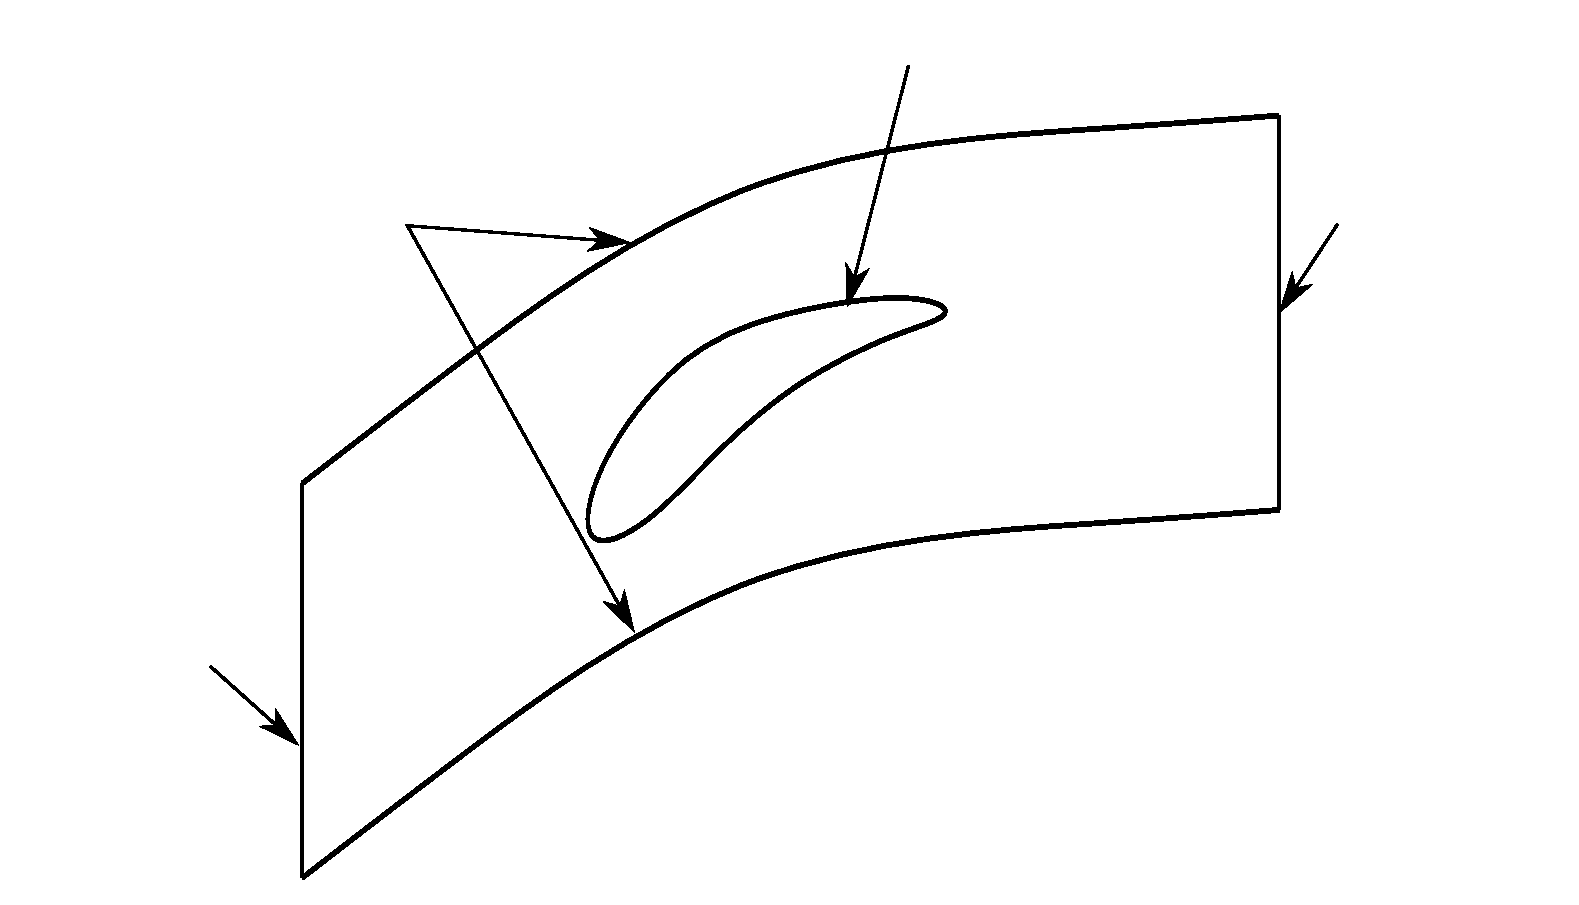
\includegraphics[width=0.7\textwidth]{img/inkscape/comp_domain.pdf}
	\caption[Topologie výpočetní oblasti]{Náčrt topologie výpočetní oblasti pro standardní axiální kompresorovou mříž.}
	\label{fig:vypocetni_oblast}
\end{figure}

Krom periodicity jsou další okrajové podmínky následující. Na vstupu je předepsána Dirichletova okrajová podmínka pro vektor rychlosti a turbulentní proměnné. Tlak zde má nulovou Neumanovu podmínku. Na výstupu je naopak statický tlak fixován na nulu a rychlost je zde předepsána pomocí nulového gradientu.

\section{Cílové funkce}

V rámci aplikace sdružené optimalizace na tvar lopatky kompresorové mříže lze vymyslet hned několik cílů. V jednom stupni axiálního kompresoru se běžně sledují veličiny stlačení, účinnost (respektive ztráty) a výstupní úhel proudu. Pro tuto práci se jako sledovaná a optimalizovaná veličina bere ta poslední, tedy výstupní úhel proudu $ \alpha_2 $. 

K dosažení cílového úhlu na výstupu z lopatkové mříže $ \alpha_{2tar} $ jsou použity dva postupy. Oba vycházejí z definice úhlu výstupního proudu
\begin{equation}\label{eq:alpha_tan}
\alpha_2 = \arctan\left(\dfrac{u_{y2}}{u_{x2}}\right).
\end{equation}
Ze zákona zachování hmotnosti pro proudění nestlačitelné tekutiny vyplývá, že to co do kontrolní oblasti vteče, musí i vytéct. Jinými slovy toky vstupní a výstupní hranicí se musejí rovnat
\begin{equation}
\dot{m_1}=\dot{m_2},
\end{equation}
což pro proudění nestlačitelné tekutiny kontrolní oblastí s vstupní a výstupní hranicí rovnoběžnou s osou y znamená, že 
\begin{equation}\label{eq:ux1_ux2}
u_{x1}=u_{x2}.
\end{equation}
Okrajové podmínky definují na vstupu konstantní uniformní vektor rychlosti $ \mathbf{u_1} $ a přeneseně tedy i x-ovou složku rychlosti na výstupu. Z toho vyplývá, že pro zadané $ \alpha_{2tar} $ můžeme apriori spočítat
\begin{equation}
u_{y2tar} = \tan(\alpha_{2tar}) \cdot u_{x2},
\end{equation}
tedy jistou cílovou rychlost na výstupu a cílovou funkci formulovat pomocí ní.

Dále jsou srovnány dvě formulace cílové funkce. První formulace optimalizuje přímo výstupní složku rychlosti, kdežto druhá optimalizuje nepřímo přes sílu na lopatku.

Zatímco přímá formulace ovlivňuje přes derivaci cílové funkce okrajovou podmínku sdružených rovnic pouze na výstupní hranici $ \Gamma_2 $, cílová funkce přes sílu ovlivňuje okrajovou podmínku na lopatce $ \Gamma_P $. Druhým rozdílem je pak, že v přímé formulaci se objevuje jediná primární proměnná, kdežto pro integraci síly na lopatce jsou potřeba všechny proměnné, včetně turbulentní proměnné $ \widetilde{\nu} $. Tyto rozdíly zavdávají dostatečný důvod pro zkoumání a porovnání těchto dvou formulací ve smyslu rychlosti konvergence a přesnosti.

\subsection{Přímá formulace}

V přímé formulaci se snažíme aby
\begin{equation}
	u_{y2tar}=\dfrac{1}{\phi_2}\sum_{f\in\Gamma_2}\phi_f u_{yf},
\end{equation}
tedy aby průměr $ u_y $ na výstupu vážený přes hmotnostní tok byl roven zadané cílové rychlosti.
Minimalizovanou cílovou funkci formulujeme jako
\begin{equation}\label{eq:J_UyTarget}
	J = \int_{\Gamma_2}\left( u_y(y)-u_{y2tar} \right)^2\mathrm{d}S = \int_{\Gamma_2} J_\Gamma\, \mathrm{d}S.
\end{equation}
Ve smyslu vztahu \ref{eq:cenova_fce} má takto definovaná cílová funkce pouze hraniční složku $ J_\Gamma $ a pro sdružené rovnice tak bude figurovat pouze v hraničních členech, tedy v rovnicích \ref{eq:sdruzenaOP1} a \ref{eq:sdruzenaOP2}. Potřebujeme tedy vydefinovat parciální derivace podle primárních proměnných $ \mathbf{u} $ a $ p $. Pro implementaci v rámci knihovny OpenFOAM je pak navíc potřeba vydefinovat ještě derivace podle $ u_n $ a $ u_t $, což pro dříve definovanou úlohu znamená podle složek $ u_x $ a $ u_y $.

Parciální derivace podle primárního tlaku $ \dfrac{\partial}{\partial p} $ je nulová, neboť tlak v cílové funkci nefiguruje.

Pro parciální derivaci podle primární rychlosti $ \mathbf{u} $ je lepší se dívat na složku $ u_y $ jako na skalární součin $ \mathbf{u}\cdot \mathbf{j}=\mathbf{u}\cdot (0,1,0) = u_y$ a derivaci tedy provést jako
\begin{equation}\label{key}
\dfrac{\partial J_\Gamma}{\partial \mathbf{u}}
=
\dfrac{\partial \left( \mathbf{u}\cdot \mathbf{j}-u_{y2tar} \right)^2}{\partial \mathbf{u}}
=
2( \mathbf{u}\cdot \mathbf{j}-u_{y2tar} )\,\mathbf{j}
=
2( u_y-u_{y2tar} )\,\mathbf{j}.
\end{equation}
U dodatečných derivací pro OpenFOAM vychází $ \dfrac{\partial}{\partial u_n}=0 $ a $ \dfrac{\partial }{\partial u_t} $ je stejná jako derivace podle $ \mathbf{u} $.

\subsection{Nepřímá formulace přes sílu}

Druhou možností jak dosáhnout zadaného úhlu výstupního proudu je použít optimalizaci přes cílovou sílu. 
Optimalizace síly na stěnu ve smyslu její minimalizace v předepsaném směru je v balíku OpenFOAM formulována jako
\begin{equation}\label{eq:J_FyOForig}
J_{OF}=\dfrac{\int_\Gamma \rho (-\tau_{ij}n_j+pn_i)r_i\,\mathrm{d}S}{\frac{1}{2}\rho A U_{\infty}^2},
\end{equation}
kde $ \tau_{ij} $ jsou složky tenzoru napětí, $ p $ tlak dělený konstantní hustotou $ \rho $ a $ \mathbf{n} $ jednotkový normálový vektor. Vektor $ \mathbf{r} $ pak definuje směr projekce vektoru síly (směr ve kterém se minimalizuje). $ A $ je referenční plocha a $ U_{\infty} $ je rychlost volného proudu. Takto definovaná cílová funkce tedy svou velikostí odpovídá koeficientu síly $ C_f $.

Pro potřeby optimalizace na cílovou sílu $ F_{yPtar} $ bylo vhodnější použít přímo samotnou sílu, tedy pouze čitatel v rovnici \ref{eq:J_FyOForig}, a za vektor projekce brát jednotkový vektor ve směru osy y. Pro celkovou sílu působící na lopatku ve směru y tak lze psát
\begin{equation}\label{key}
F_{yP}=\int_{\Gamma_P} \rho (-\tau_{ij}n_j+pn_i)\delta_{i2}\,\mathrm{d}S.
\end{equation}
Absolutní velikost takto vyhodnocené síly samozřejmě závisí i na rozměru lopatky v ose z. Číselné výsledky uváděné později jsou uváděny vždy relativní, takže nezávisí na libovolné konstantní výšce lopatky. Cílovou funkci pro cílovou sílu tak definujeme podobně jako pro rychlost přes kvadrát rozdílu, tedy
\begin{equation}\label{eq:J_FyTarget}
J= (F_{yP} - F_{yPtar})^2.
\end{equation}
Pro derivaci této cílové funkce podle libovolné proměnné $ w $ pak platí
\begin{equation}\label{key}
\dfrac{\partial J}{\partial w} = 
2(F_{yP}-F_{yPtar}) \cdot \dfrac{\partial F_{yP}}{\partial w}.
\end{equation}
Výraz $ \frac{\partial F_{yP}}{\partial w} $ odpovídá derivaci čitatele (anglicky \textit{nominator}, $ \mathrm{nom()} $) cílové funkce definované rovnicí \ref{eq:J_FyOForig}, tedy
\begin{equation}\label{key}
\dfrac{\partial F_{yP}}{\partial w} = \dfrac{\partial (\mathrm{nom}(J_{OF}))}{\partial w}.
\end{equation}
Pro tuto cílovou funkci tedy nebylo potřeba odvozovat potřebné derivace a stačilo pouze vynásobit příslušné výrazy definované v kódu knihovny OpenFOAM výrazem $ 2(F_{yP}-F_{yPtar}) $.



\section{Optimalizace mříže GHH 1-S1}
Pro aplikaci nově zpracovaných cílových funkcí byla zvolena axiální kompresorová mříž MAN GHH 1-S1 publikovaná v \cite{steinert1990design}.
Výpočetní oblast topologicky odpovídá náčrtu na obrázku \ref{fig:vypocetni_oblast}.
Rozteč lopatek v mříži je $ t=0.0476\,\mathrm{m} $. Hustota tekutiny používaná při vyhodnocení síly je $ \rho=1.225\,\mathrm{kg\,m^{-3}} $ a kinematická viskozita $ \nu = 1.5\cdot10^{-5} \, \mathrm{m^2s^{-1}} $.

\subsection{Okrajové podmínky}  Na vstupu je Machovo číslo $ M=0.62 $ a úhel proudu $ \alpha_1 = 47^\circ $, což při klidové rychlosti vzduchu $ c=340 \,\mathrm{m\,s^{-1}} $ vede na okrajovou podmínku pro vstupní rychlost  
\begin{equation}\label{key}
\mathbf{u_1}=M\cdot c \cdot (\cos(\alpha_1),\, \sin(\alpha_1),\, 0) \doteq (143.8,\, 154.2,\, 0)\, \mathrm{m\,s^{-1}}.
\end{equation}
Kinematický tlak na výstupu je fixován $ p_2=0\,\mathrm{m^2s^{-2}} $.

\subsection{Modelování turbulence}
Modelování turbulence se realizuje pomocí přídavné turbulentní vazkosti. Pro zjištění turbulentní vazkosti $ \nu_t $ je v optimalizačním algoritmu použit model Spalart-Allmaras\cite{spalart1992one}. Jelikož ale tento model je původně navržen pro obtékání profilu křídla ve volném proudu, není ve své původní variantě vhodný pro modelování turbulence ve vnitřní aerodynamice, kam kompresorové mříže spadají. Knihovna OpenFOAM prozatím ale neobsahuje sdružené rovnice pro žádný jiný model turbulence než Spalart-Alamaras a odvození sdružených rovnic pro pokročilejší model turbulence je nad rámec této práce, byl použit následující postup. 

Ve výchozí konfiguraci byla provedena simulace s vhodnějším modelem $k\text{-}\omega$ SST implementovaným v knihovně OpenFOAM na základě \cite{menter1994two, menter2003ten, rumsey2013menter} s následujícími okrajovými podmínkami na vstupu. Intenzita turbulence na vstupu $ I=2\% $, tedy odkud plyne Dirichletova podmínka pro turbulentní kinetickou energii $ k $ ze vztahu  \begin{equation}\label{key}
k=1.5(I|\mathbf{u}|)^2.
\end{equation} 
Turbulentní směšovací délka $ L_t=0.002\,\mathrm{m} $, odkud plyne Dirichletova okrajová podmínka pro $ \omega $ ze vztahu
\begin{equation}\label{key}
\omega=\dfrac{k^{0.5}}{C_\mu^{0.25}L_t};\,\, C_\mu=0.09\,.
\end{equation} 
Ve výchozí konfiguraci bylo následně provedeno několik simulací s modelem Spalart-Allmaras, kde se variovala vstupní hodnota turbulentní proměnné tohoto modelu $ \tilde{\nu}_1 $ z intervalu $ \langle 10^{-6},10 \rangle $. Pro každý výpočet byl vyhodnocen koeficient ztráty celkového tlaku podle vztahu z \cite{steinert1990design}
\begin{equation}\label{key}
\omega = \dfrac{p_{t1}-p_{t2}}{p_{t1}-p_1}
\end{equation}
a poměr celkových tlaků $ \frac{p_{t1}}{p_{t2}} $. Pro další simulace této lopatkové mříže pak byla na vstupu zvolena Dirichletova podmínka $ \tilde{\nu} = 3.4\cdot 10^{-4} $ neboť pro tuto hodnotu vyšel relativní rozdíl v předpovědi modelem Spalart-Allmaras oproti $k\text{-}\omega$ SST pro obě vyhodnocované veličiny pod $ 1\% $.

\subsection{Prostorová diskretizace}

Výpočetní oblast byla diskretizována na množinu vzájemně disjunktních objemů. Dvourozměrná síť byla vytvořena v softwaru ANSYS ICEM a její detail je ukázán na obrázku \ref{fig:ghs1_sit}. Následný převod sítě do formátu pro OpenFOAM (2D síť na pseudo-3D) byl proveden s parametrem 0.01 pro souřadnice $ z $.

\begin{figure}
	\centering
	\def\svgwidth{1\textwidth}
	\graphicspath{{img/inkscape/}}
	\includesvg{img/inkscape/wireframe}
	\caption[Výpočetní síť mříže GHH 1-S1]{Výpočetní síť pro lopatkovou mříž GHH 1-S1 s detailem náběžné a odtokové hrany. Síť sestává z celkem 85 tisíc hexahedrálních buněk. }
	\label{fig:ghs1_sit}
\end{figure}

Síť byla tvořena s důrazem na co nejlepší zachycení mezní vrstvy. Buňky v oblasti okolo lopatky jsou exponenciálně zmenšovány, aby se dosáhlo $ y^+ < 1 $ a nebylo tak nutné používat stěnové funkce ani pro jeden z turbulentních modelů.
S touto sítí ve výchozí konfiguraci s modelem $k\text{-}\omega$ SST je dosaženo $ \max\limits_{\Gamma_P}(y^+) \doteq 0.39 $. Validita této sítě byla ověřena metodou \textit{Grid convergence index} (zkráceně GCI) v \cite{tater2021mesh}.


\subsubsection{Řídící body objemových B-spline}
Pro transformaci tvaru lopatky a pohybu se sítí pomocí objemových B-spline je potřeba vydefinovat řídící body. Z experimentů s různým rozdělením řídících bodů a jejich fixací v průběhu optimalizačních cyklů vzešlo, že stabilita řešení sdružených rovnic i konečný výsledek optimalizace na rozdělení řídících bodů závisí víc než by se dalo označit za uživatelsky příjemné. Konečné rozdělení řídících bodu je ukázáno na \ref{fig:ghs1_cps}. Ve směru $ u $, který koresponduje se směrem osy $ x $, bylo zvoleno 14 vrstev bodů a ve směru $ v $ pak 6. Fixované v průběhu simulace byly všechny krajní body. Druhá a předposlední vrstva ve směru $ u $ (sloupec) má pak zakázán pohyb ve směru osy $ x $. Vrstvy ve směru $ u $ procházející náběžnou a odtokovou hranou profilu mají zakázán pohyb úplně. Cílem těchto omezení je fixovat pozici začátku a konce lopatky, aby nedošlo k natahování lopatky a deformaci odtokové hrany. Tento nechtěný efekt měl tendenci nastat pokud se fixovaly například pouze vnější body.

\begin{figure}
	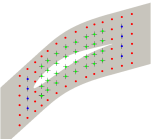
\includegraphics[width=0.75\textwidth]{img/cps.png}
	\caption[Pozice řídících bodů]{Pozice řídících bodů objemových B-spline ve výpočetní oblasti pro lopatkovou mříž GHH 1-S1. Růžové body se smí pohybovat pouze ve směru osy $ y $.}
	\label{fig:ghs1_cps}
\end{figure}


\subsection{Parametry optimalizace}
Cílové funkce používané pro optimalizaci jsou definovány rovnicemi \ref{eq:J_UyTarget} a \ref{eq:J_FyTarget}, tedy optimalizace přímá na $ u_{y2tar} $ a nepřímá na $ F_{yPtar} $. Optimalizace tvaru lopatky byla dodatečně omezena, tak aby průřez lopatky zůstal konstantní, což lze pro trojrozměrný prostor matematicky formulovat jako
\begin{equation} 
V=-1/3\int_{\Gamma_P}x_kn_k\mathrm{d}S.
\end{equation}

Kvůli přidané podmínce konstantního průřezu byla jako metoda aktualizace zvolena metoda projekce omezení (anglicky \textit{constraint projection}). Výchozí krok ve směru gradientu $ \eta $ je v první iteraci spočítán podle maximálního povoleného pohybu sítě, který byl nastaven na $ 5\cdot10^{-4} $. Velikost kroku $ \eta $ se posléze v jednotlivých iteracích zmenšuje podle Armijo podmínky jak definuje \cite{nocedal1999numerical}. Tento cyklus zmenšuje krok $ \eta^{k+1}=0.75\cdot\eta^{k} $ a vyhodnocuje hodnotu cílové funkce $ J $ (tedy simuluje primární rovnice), než jsou splněny dané podmínky. Pro Armijo podmínky je důležitý koeficient $ c1 $, který byl zvolen $ 10^{-3} $.

Výstupní úhel proudu byl ve výchozí konfiguraci s modelem Spalart-Allmaras $ \alpha_{2}^{0}=21.46^{\circ} $. Cílové výstupní úhly byly zvoleny z množiny $ \langle \alpha_{2}^{0}-4^{\circ}, \alpha_{2}^{0}+8^{\circ} \rangle $ s krokem $ 2^{\circ} $. Celkem tedy 6 různých cílových úhlů.

\subsection{Výsledky optimalizace} \label{sec:vysledky_opt}
K dosažení cílového úhlu výstupního proudu byla použita nejdříve přímá formulace cílové funkce. Následně, když optimalizace bylo nalezeno optimální řešení, byla vyhodnocena síla $ F_{yP} $ působící na lopatku. Tato síla pak byla použita jako cílová síla $ F_{yPtar} $ pro nepřímou formulaci cílové funkce. Konkrétní cílové hodnoty s odpovídajícími cílovými úhly jsou uvedeny v tabulce \ref{tab:cilove_hodnoty}.

\begin{table}
	\begin{ctucolortab}
		\begin{tabular}{c|c||c|c}
			
			$ \Delta\alpha_{2} $ &$ \alpha_{2tar} $ & $ u_{y2tar}\,[\mathrm{ms^{-1}}] $ & $ F_{yPtar}\,[\mathrm{N}] $ \\
			\hline
			-4° & 17.46° & 45.32 & 9.12 \\
			
			-2° & 19.46° & 50.91 & 8.65 \\
			
			+2° & 23.46° & 62.53 & 7.69 \\
			
			+4° & 25.46° & 68.60 & 7.17 \\
			
			+6° & 27.46° & 74.87 & 6.65 \\
			
			+8° & 29.46° & 81.38 & 6.10 \\
			
		\end{tabular}
	\end{ctucolortab}
	\caption{Cílové hodnoty pro optimalizaci.}
	\label{tab:cilove_hodnoty}
\end{table}

\subsubsection{Optimalizace $ u_{y2} $}


Pro vyhodnocení konvergence optimalizace s přímou formulací cílové funkce je jako určující norma (residuum) pro každou iteraci $ i $ brán relativní rozdíl
\begin{equation}\label{eq:res_uy}
Res_{u_{y}}^i=\dfrac{|u_{y2}^i-u_{y2tar}|}{|u_{y2}^0|}.
\end{equation}
Residua pro všechny cílové hodnoty v průběhu optimalizačních cyklů jsou ukázány na obrázku \ref{fig:ghs1_Uy}.
Optimalizaci pak považujeme za zkonvergovanou, pokud residuum klesne pod jedno procento. Na obrázku \ref{fig:ghs1_Uy} je hranice konvergence naznačena růžovou čarou.

Jelikož ale ve výsledku chceme optimalizovat hodnotu výstupního úhlu, je rozumné se dívat i na residuum vzhledem k $ \alpha_2 $, tedy na 
\begin{equation}\label{eq:res_alpha}
Res_{\alpha}^i=\dfrac{|\alpha_{2}^i-\alpha_{2tar}|}{|\alpha_{2}^0|}.
\end{equation}
Graf residuí $ Res_{\alpha}^i $ na obrázku \ref{fig:ghs1_UyA} je samozřejmě pro přímou formulaci velice podobný grafu residua samotné optimalizace, neboť $ \alpha_2 $ se z $ u_{y2} $ přímo vyhodnocuje podle vztahu \ref{eq:alpha_tan}. Teoreticky by měly být grafy naprosto stejné, neboť $ u_{x2} $ by mělo být podle vztahu \ref{eq:ux1_ux2} pro všechny případy stejné. Vlivem chyb diskretizace tomu tak úplně není a grafy se tak pro malé hodnoty residua drobně liší.

Dále lze z grafu residuí vypozorovat, že čím větší je rozdíl $ \Delta \alpha_{2} = \alpha_{2tar} - \alpha_{2}^{0}$, tím déle trvá optimalizaci zkonvergovat. To samozřejmě odpovídá očekávání. Při porovnání rychlosti konvergence optimalizace do záporných versus do kladných úhlu výstupního proudu lze říci, že optimalizovat do kladných úhlů je pro takto nastavený optimalizační algoritmus jednodušší. Optimalizace do kladných úhlů odpovídá napřimování tvaru lopatky, kdežto při optimalizaci do záporných úhlů je pro dosažení cílové hodnoty úhlu výstupního proudu potřeba lopatku ohnout více. Tento zmiňovaný rozdíl lze nejlépe vidět při porovnání případů $ \alpha_{2tar}=\pm 4^{\circ} $. Pro kladný úhel +4° je optimální řešení nalezeno už v 9. iteraci, kdežto při ohýbání lopatky k dosažení záporného $ \Delta\alpha $ je potřeba optimalizačních cyklů 12.

\begin{figure}[H]
	\includegraphics[width=0.95\textwidth]{img/Uy.pdf}
	\caption[Průběh residua $ Res_{u_y}^i $]{Průběh residua $ Res_{u_y}^i $ \ref{eq:res_uy} pro přímou formulaci cílové funkce $ J $ v průběhu iteračních cyklů. Hranice optimálního řešení $ 1\% $ je naznačena růžovou čarou.}
	\label{fig:ghs1_Uy}
\end{figure}

\begin{figure}[H]
	\includegraphics[width=0.95\textwidth]{img/Fy.pdf}
	\caption[Průběh residua $ Res_{F_y}^i $]{Průběh residua $ Res_{F_y}^i $ \ref{eq:res_fy} pro nepřímou formulaci cílové funkce $ J $ v průběhu iteračních cyklů. Hranice optimálního řešení $ 1\% $ je naznačena růžovou čarou.}
	\label{fig:ghs1_Fy}
\end{figure}

\subsubsection{Optimalizace $ F_{yP} $}

Pro vyhodnocení optimálnosti řešení pro nepřímou formulací cílové funkce je jako residuum pro každou iteraci $ i $ brán relativní rozdíl
\begin{equation}\label{eq:res_fy}
Res_{F_{y}}^i=\dfrac{|F_{yP}^i-F_{yPtar}|}{|F_{yP}^0|}.
\end{equation}
Stejně jako pro přímou formulaci bereme hranici optimálního řešení jedno procento. Residua pro všechny cílové hodnoty v průběhu optimalizačních cyklů pro nepřímou formulaci cílové funkce jsou ukázány na obrázku \ref{fig:ghs1_Fy} s naznačenou hranicí konvergence. 

V porovnání s grafem konvergence \ref{fig:ghs1_Uy} pro přímou formulaci cílové funkce průběh residua \ref{fig:ghs1_Fy} o poznání méně osciluje. To si lze vysvětlit tím, že pro vyhodnocení cílové funkce pro sílu (a jejích derivací) jsou použity všechny primární proměnné a tedy se využívá více informací z proudového pole pro předpověď gradientu. Na základě tohoto pozorování lze s opatrností usoudit, že optimalizace na cílovou sílu je značně stabilnější než optimalizace na cílovou výstupní rychlost. Zároveň optimalizační algoritmus zkonverguje v méně iteracích než tomu bylo pro přímou formulaci cílové funkce. Například pro případ $ \Delta \alpha = +8^\circ $ stačilo o pět iterací méně. V tomto smyslu by bylo zajímavé i porovnání průběhu residuí jako funkce výpočetního času. V současné konfiguraci optimalizačních algoritmů byl celkový čas výpočtu (pro 50 iterací) vždy nižší pro přímou formulaci. Ve zmiňovaném případě $ \Delta \alpha = +8^\circ $ byl celkový výpočetní čas pro přímou formulaci $ 2265 \,\mathrm{s} $ a pro nepřímou formulaci $ 2927 \,\mathrm{s} $.

\begin{figure}[H]
	\includegraphics[width=0.9\textwidth]{img/UyA.pdf}
	\caption[Průběh residua $ Res_{\alpha}^i $, přímá formulace]{Průběh residua $ Res_{\alpha}^i $ \ref{eq:res_alpha} pro přímou formulaci cílové funkce $ J $ v průběhu iteračních cyklů. Hranice optimálního řešení $ 1\% $ je naznačena růžovou čarou.}
	\label{fig:ghs1_UyA}
\end{figure}

\begin{figure}[H]
	\includegraphics[width=0.9\textwidth]{img/FyA.pdf}
	\caption[Průběh residua $ Res_{\alpha}^i $, nepřímá formulace]{Průběh residua $ Res_{\alpha}^i $ \ref{eq:res_alpha} pro nepřímou formulaci cílové funkce $ J $ v průběhu iteračních cyklů. Hranice optimálního řešení $ 1\% $ je naznačena růžovou čarou.}
	\label{fig:ghs1_FyA}
\end{figure}

Optimalizaci na cílovou sílu používáme k nepřímému dosažení žádaného výstupního úhlu proudu. Proto je důležitější podívat se na graf konvergence ve smyslu vztahu \ref{eq:res_alpha}, který je na obrázku \ref{fig:ghs1_FyA}. Nejmarkantnějším rozdílem v porovnání s grafem \ref{fig:ghs1_UyA} je průběh residua pod hranicí konvergence, který je opět hladší. Nejdůležitější srovnání je ale v počtu iterací potřebných ke zkonvergování $ \alpha_2 $. Na rozdíl od porovnání cílových residuí $ Res_{u_y}^i $ a $ Res_{F_y}^i $ je počet potřebných iterací pro všechny případy $ \Delta\alpha_2 $ stejný. Jak bylo ale zmíněno v předchozím odstavci, optimalizace s přímou formulací cílové funkce je ve všech případech rychlejší. Na základě tohoto porovnání lze bezpečně říci, že pro případ optimalizace lopatky GHH 1-S1 na takto kvalitní síti nepřináší nepřímá formulace žádné benefity. Pro jiné případy tomu tak ovšem být nemusí, neb z průběhu cílových residuí \ref{eq:res_uy} a \ref{eq:res_fy} lze usoudit, že optimalizace na cílovou sílu je mnohem stabilnější, což může hrát ve složitějších aplikacích důležitou roli.
\newpage
\subsubsection{Srovnání pro $ \Delta \alpha_2=-4^{\circ} $}

Porovnání tvaru lopatky je provedeno mezi původním tvarem profilu a profilem z optimalizace zkorvergované ve smyslu $ Res_{\alpha}^i $. Pro $ \alpha_2=-4^\circ $ to je profil ze 12. iterace optimalizačního algoritmu.

\begin{figure}[H]
	\centering
	\def\svgwidth{0.8\textwidth}
	\graphicspath{{img/inkscape/}}
	\includesvg{img/inkscape/prof_wire}
	\caption[Tvar optimalizované lopatky]{Obrys tvaru lopatky před optimalizací (černě) a po optimalizaci s přímou (modře) a nepřímou (červeně) formulací cílové funkce. Červená křivka na většině obrázku překrývá modrou.}
	\label{fig:ghs1_alphaminus4}
\end{figure}

\begin{figure}[H]
\includegraphics[width=0.75\textwidth]{img/displacement_12.png}
\caption[Pole posunutí sítě]{Vizualizace pole posunu bodů sítě ve směru osy $ y $.}
\label{fig:ghs1_disp12}
\end{figure}

Zajímavé je srovnání optimalizovaných tvarů lopatky získaných přímou a nepřímou formulací. Jak je vidět na obrázku \ref{fig:ghs1_alphaminus4}, tvar optimalizovaných profilu je v podstatě totožný. Obě formulace pohybují především s částí lopatky v blízkosti odtokové hrany jak je vidět z obrázku \ref{fig:ghs1_disp12}. To dává smysl, neboť koncová část lopatky má často mnohem větší vliv na směr proudu na výstupu než část u náběžné hrany.
\begin{figure}[h]
	\includegraphics[width=0.7\textwidth]{img/magU_0.png}
	\caption[Velikost rychlosti pro původní lopatku]{Pole velikosti vektoru rychlosti $ ||\mathbf{u}|| $ pro původní profil lopatky.}
	\label{fig:ghs1_U0}
\end{figure}
\begin{figure}[h]
	\includegraphics[width=0.7\textwidth]{img/magU_12.png}
	\caption[Velikost rychlosti pro optimalizovanou lopatku]{Pole velikosti vektoru rychlosti $ ||\mathbf{u}|| $ pro optimalizovaný profil lopatky.}
	\label{fig:ghs1_U12}
\end{figure}

Pro detailnější představu o vlivu změny tvaru lopatky je nyní uvedeno několik obrázků.
Nejprve lze porovnat pole velikosti rychlosti pro původní \ref{fig:ghs1_U0} a optimalizovaný \ref{fig:ghs1_U12} tvar lopatky. 
Za koncem lopatky lze vidět pruh nižší velikosti rychlosti, což je úplav. Směr úplavu vizuálně naznačuje směr proudu na výstupu. Při porovnání stavu před a po lze jasně vidět, že směr úplavu změnil. Přesněji se proud ohnul dolů, což odpovídá zmenšení úhlu proudu na výstupu. Zároveň je u optimalizované lopatky vidět větší oblast odtržení proudu u odtokové hrany. Tento efekt potvrzuje i porovnání pole přídavné turbulentní vazkosti $ \nu_t $ na obrázcích \ref{fig:ghs1_nut0} a \ref{fig:ghs1_nut12}. 
\begin{figure}[h]
	\includegraphics[width=0.7\textwidth]{img/nut_0.png}
	\caption[Turbulentní vazkost pro původní lopatku]{Pole přídavné turbulentní vazkosti $ \nu_t $ pro původní profil lopatky $ \alpha_{2}=\alpha_2^0 $.}
	\label{fig:ghs1_nut0}
\end{figure}
\begin{figure}[h]
	\includegraphics[width=0.7\textwidth]{img/nut_12.png}
	\caption[Turbulentní vazkost pro optimalizovanou lopatku]{Pole přídavné turbulentní vazkosti $ \nu_t $ pro optimalizovaný profil lopatky.}
	\label{fig:ghs1_nut12}
\end{figure}
Maximální velikost přídavné vazkosti v oblasti úplavu za optimalizovanou lopatkou je vyšší a úplav jako takový je širší. To ve výsledku vede na větší ztráty, což dokládá například i zvýšení velikosti síly působící na lopatku ve směru osy $ x $. Optimalizovaná lopatka tedy splňuje cílové ohnutí proudu, z hlediska účinnosti ale tento tvar optimální neníx.
%\begin{figure}
%	\centering
%	\begin{minipage}[t]{0.48\textwidth}
%		\centering
%		\includegraphics[width=1\textwidth]{img/magU_0.png}
%	\end{minipage}
%	\hfill
%	\begin{minipage}[t]{0.48\textwidth}
%		\centering
%		\includegraphics[width=1\textwidth]{img/magU_12.png}
%	\end{minipage}
%	\caption{Pole velikosti vektoru rychlosti pro původní (vlevo) a optimalizovaný (vpravo) profil lopatky.}
%	\label{fig:ghs1_U}
%\end{figure}
%
%\begin{figure}
%\centering
%\begin{minipage}[t]{0.48\textwidth}
%	\centering
%	\includegraphics[width=1\textwidth]{img/nut_0.png}
%\end{minipage}
%\hfill
%\begin{minipage}[t]{0.48\textwidth}
%	\centering
%	\includegraphics[width=1\textwidth]{img/nut_12.png}
%\end{minipage}
%\caption{Pole přídavné turbulentní vazkosti pro původní (vlevo) a optimalizovaný (vpravo) profil lopatky.}
%\label{fig:ghs1_nut}
%\end{figure}


\subsection{Ověření vhodnějším modelem turbulence}

Pro ověření výsledků optimalizace byl zvolen model $k\text{-}\omega$ SST, který je pro simulace v kompresorech i lopatkových mříží vhodnější než model Spalart-Allmaras. Nejdříve budou ukázány grafy residuí a následně bude podrobněji rozebrán případ $ \Delta \alpha = -4^\circ $.

Pro vyhodnocení residua $ Res_\alpha^{iSST} $ (horní index $ \null^{SST} $ značí vyhodnocení ze simulace s modelem $k\text{-}\omega$ SST) na obrázcích \ref{fig:ghs1_UyAKO} a \ref{fig:ghs1_FyAKO} je na rozdíl od $ Res_\alpha^i $ definovaném rovnicí \ref{eq:res_alpha} použito pro vyhodnocení $ \alpha_{2}^{0SST} $ namísto $ \alpha_{2}^{0} $, tedy
\begin{equation}\label{eq:res_alphaSST}
Res_\alpha^{iSST} = \dfrac{| \alpha_{2}^{iSST}-( \alpha_{2}^{0SST}+\Delta\alpha_2 ) |} {|\alpha_{2}^{0SST}|}.
\end{equation}
Na základě grafů průběhu residua \ref{fig:ghs1_UyAKO} a \ref{fig:ghs1_FyAKO} lze říci, že přestože se v rámci optimalizačního cyklu používá jednodušší model turbulence, tak nový tvar lopatky funguje pro změnu úhlu $ \Delta\alpha\in\langle -2^\circ,+4^\circ\rangle $ i v případě simulace s vhodnějším modelem. Pro větší změny úhlu, konkrétně $ -4^\circ $ a $ +8^\circ $, je ale natočení proudu nesprávné. Pro záporné změny úhlu je tedy předpověď modelu Spalart-Allmaras horší než pro kladné změny úhlu.
Částečné vysvětlení tohoto rozdílu plyne z obrázku \ref{fig:ghs1_sakoUdiff}, který ukazuje relativní rozdíl velikosti rychlosti předpovídané modelem turbulence Spalart-Allmaras ($ \null^{S\text{-}A} $) a $k\text{-}\omega$ SST ($ \null^{SST} $), podle předpisu
\begin{equation}\label{eq:ghs1_sakoUdiff}
\dfrac{||\mathbf{u^{S\text{-}A}||-||u^{SST}}||}{||\mathbf{u_1}||}.
\end{equation}
Největší rozdíl je v blízkosti odtokové hrany na podtlakové straně, kde dochází k odtržení proudu. Simulace s modelem Spalart-Allmaras zde předpovídá mnohem větší velikost rychlosti a lze tedy usoudit, že nezachycuje odtržení správným způsobem. Z obrázku \ref{fig:ghs1_sakoUdiff} je mimo jiné vidět, že výpočet s modelem $k\text{-}\omega$ SST předpovídá, že změna úhlu proudu bude větší než žádané 4°. Z grafu průběhu residua předtím nešlo říct, jestli je podle $k\text{-}\omega$ SST ohnutí proudu větší či menší, protože rozdíl v čitateli je v absolutní hodnotě.
\begin{figure}[H]
	\centering
	\includegraphics[width=0.95\textwidth]{img/UyAKO.pdf}
	\caption[ Průběh residua $ Res_{\alpha}^{iSST} $, přímá formulace, $k\text{-}\omega$ SST ]{Průběh residua $ Res_{\alpha}^{iSST} $ \ref{eq:res_alpha} pro přímou formulaci cílové funkce $ J $ v průběhu iteračních cyklů. Hranice optimálního řešení $ 1\% $ je naznačena růžovou čarou. Výpočty používají model turbulence $k\text{-}\omega$ SST.}
	\label{fig:ghs1_UyAKO}
\end{figure}
\begin{figure}[H]
	\centering
	\includegraphics[width=0.95\textwidth]{img/FyAKO.pdf}
	\caption[ Průběh residua $ Res_{\alpha}^{iSST} $, nepřímá formulace, $k\text{-}\omega$ SST ]{Průběh residua $ Res_{\alpha}^{iSST} $ \ref{eq:res_alpha} pro nepřímou formulaci cílové funkce $ J $ v průběhu iteračních cyklů. Hranice optimálního řešení $ 1\% $ je naznačena růžovou čarou. Výpočty používají model turbulence $k\text{-}\omega$ SST.}
	\label{fig:ghs1_FyAKO}
\end{figure}
\begin{figure}[H]
\centering
\includegraphics[width=0.95\textwidth]{img/sako_magUdiff.png}
\caption[Rozdíl rychlosti pro modely turbulence]{
Rozdíl velikosti rychlosti pro simulaci s modelem Spalart-Allmaras a s modeleme $k\text{-}\omega$ SST. V červené oblasti předpovídá simulace $ \null^{S\text{-}A} $ vyšší velikost rychlosti, v modré oblasti pak menší, než simulace $ ^{SST} $.}
\label{fig:ghs1_sakoUdiff}
\end{figure}







